\chapter{Démarche}
\label{ch:demarche}

\PartialToc

Créer des modèles d'architecture d'entreprise à des fins d'analyse par simulation implique de suivre un processus précis. L'objectif de notre travaux est de définir le processus de modélisation et de simulation à adopter, les rôles impliqués, les artefacts conceptuels requis, ainsi que les outils et les langages adéquats pour mener des analyses de structure et de comportement. 

Notre contribution est double. D'abord, nous proposons une démarche de modélisation et d'analyse qui s'appuie sur un cadre d'architecture multi-vues. Nous dotons ce cadre d'architecture d'une vue supplémentaire qui est est la vue intégration. Cette vue a pour but d'adresser les problématiques de cohérence et d'alignement. Ensuite, nous mettons à profit les langages et standards de l'IDM permettant de modéliser et de simuler les architectures d'entreprise. 


%In this section, we present our approach and we apply it on the case study of managing an electric vehicles fleet. Our contribution is twofold. First, we propose a multi-view framework for EA with an additional view: the integration view. This view aims to address consistency and alignment issues. Second, we use executable and standardized languages from MDE to model and simulate EA.


\section{Approche conceptuelle pour la modélisation et l'analyse d'architectures d'entreprise}

L'EA peut avoir différents objectifs. Kurpjuweit et Winter \cite{kurpjuweit2007viewpoint} identifient trois objectifs de l'EA par rapport aux SI de l'entreprise~:~(1)~la documentation et la communication, (2)~l'analyse et la compréhension et (3)~la conception. Nous étendons cette vision centrée sur les SI à l'ensemble de l'entreprise en adoptant l'école de pensée «~intégrative~» comme décrite par la taxonomie de Lapalme (voir section \ref{Lapalme}, page \pageref{Lapalme} de l'état de l'art). 

Nous considérons donc que la documentation et la communication, l'analyse et la compréhension et enfin la conception concernent tout le système entreprise et pas seulement sa composante SI. Par exemple, contrairement à une EA centrée sur les SI, les processus métier sont modélisés et évalués tout autant que l'architecture applicative. La figure \ref{fig:approche_conceptuelle} illustre notre approche conceptuelle. Celle-ci fait intervenir plusieurs types d'acteurs intervenant à plusieurs niveaux de l'entreprise~:
\begin{itemize}
\item un analyste métier qui conçoit la vue métier à travers la modélisation et l'évaluation des processus métier mettant en œuvre la stratégie de l'entreprise~;
\item un architecte fonctionnel qui traduit les processus métier en termes de fonctions logiques~;
\item un architecte applicatif qui traduit la vue fonctionnelle en un ensemble structuré d'applications implémentant les différentes fonctions~;
\item un architecte d'entreprise dont la mission est de mettre en cohérence l'ensemble des vues.
\end{itemize}

\begin{figure}[!ht]
 \begin{center}
  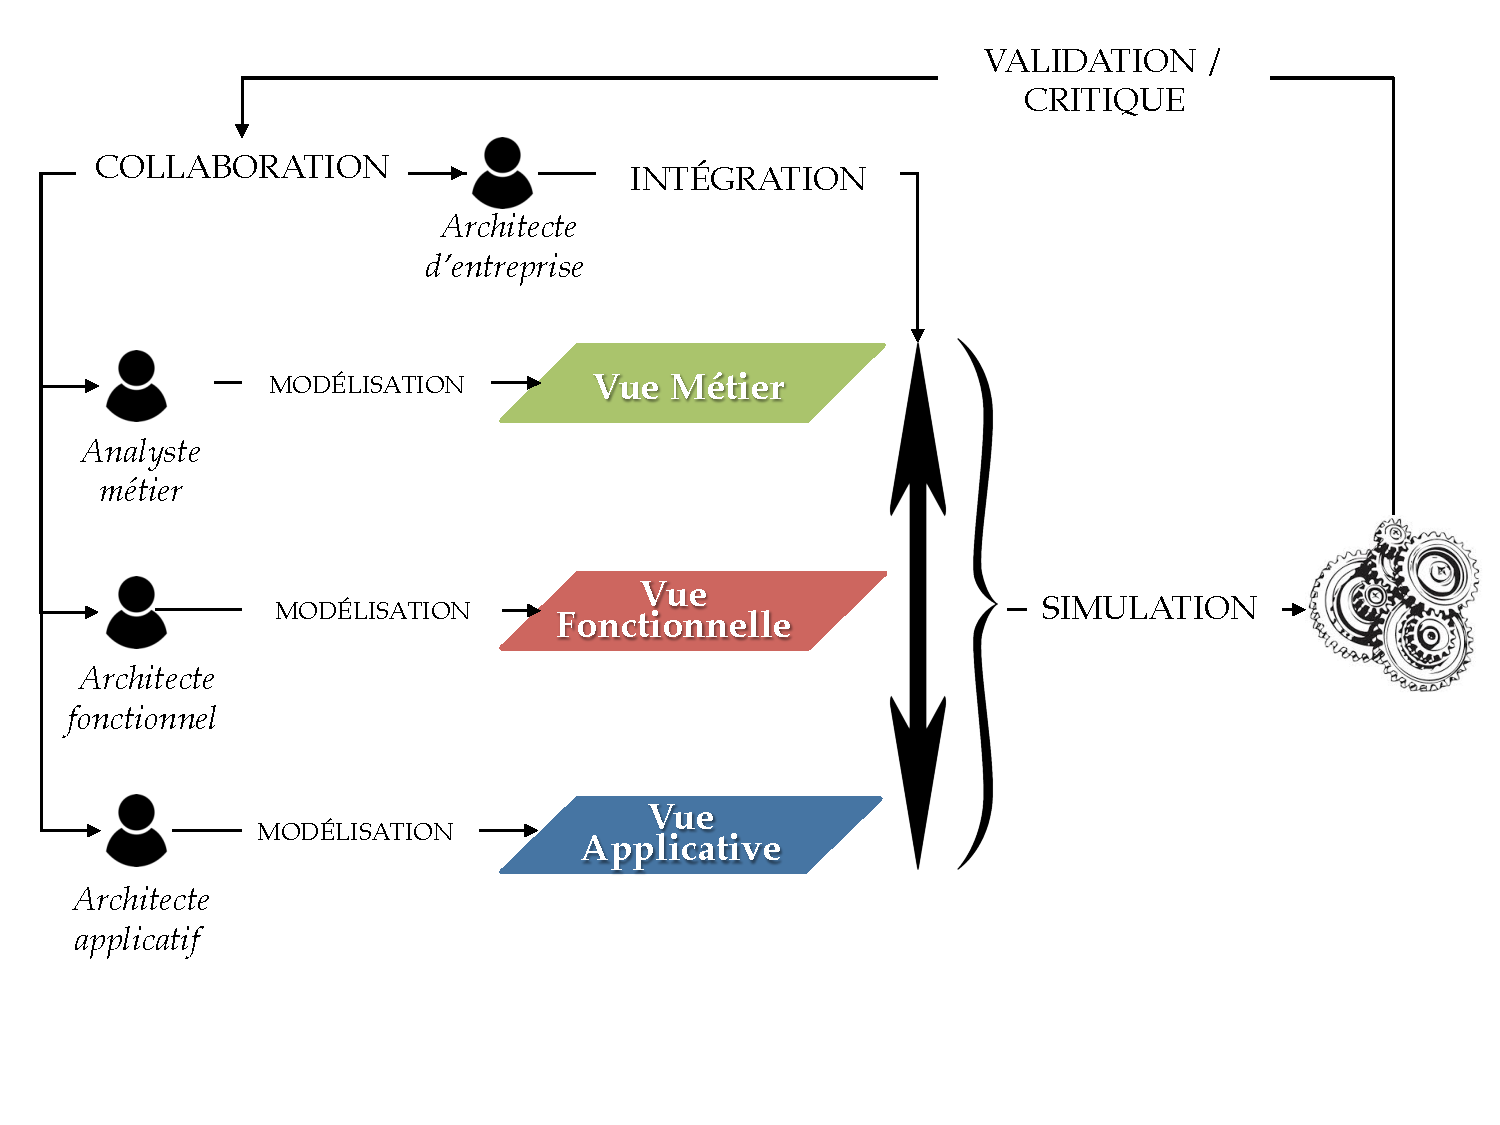
\includegraphics[trim= 0cm 3.5cm 0cm 0cm, width=1\textwidth]{figures/4_demarche/approche_conceptuelle.pdf}
 \end{center}
 \caption{Approche conceptuelle pour l'analyse d'une architecture d'entreprise}
 \label{fig:approche_conceptuelle}
\end{figure}

L'analyste métier, l'architecte fonctionnel et l'architecte applicatif collaborent entre eux et avec l'architecture d'entreprise pendant tout le processus de modélisation. Par la suite, l'activité d'intégration incombe à l'architecte d'entreprise, détenteur de la vision globale. Mais l'intégration des vues implique de rebouclage avec les autres acteurs (analyste métier, architecte fonctionnel et architecte applicatif) pour garantir l'alignement business/IT. Les étapes de modélisation et d'intégration de notre approche répondent donc aux objectifs de conception et de communication tels que définis par Kurpjuweit et Winter \cite{kurpjuweit2007viewpoint}.

Comme relaté dans l'état de l'art, l'analyse fait partie des activités les moins courantes de l'EA quelle qu'en soit l'école de pensée \cite{chen2008architectures} \cite{barn2013enterprise}. Et même lorsqu'une architecture d'entreprise est analysée très peu d'approches recourent à la simulation pour analyser l'aspect comportemental \cite{glazner2011enterprise} \cite{manzur2015xarchimate}. La simulation est pourtant une technique reconnue pour évaluer le comportement d'un système et/ou évaluer plusieurs stratégies concernant son fonctionnement \cite{shannon1975systems}. Notre approche préconise de simuler les modèles issus de activités de modélisation et d'intégration afin de les valider ou les critiquer par l'ensemble des acteurs impliqués dans l'EA. Nous couvrons ainsi l'objectif d'analyse tel que préconisé par Kurpjuweit et Winter \cite{kurpjuweit2007viewpoint}. 



\section{Un cadre d'architecture dirigé par les modèles exécutables}

\subsection{Approche par points de vue}

Toute simulation d'un système commence par sa modélisation. Pour modéliser des systèmes complexes comme les architectures d'entreprise, nous adoptons une approche par points de vue. Celle-ci facilite la conception des modèles par les acteurs impliqués en séparant leurs préoccupations respectives. Elle permet également de présenter les modèles obtenus, ainsi que les résultats de simulation de manière plus compréhensible à ces acteurs, car chaque point de vue n'utilise que les concepts métier propres à chaque acteur, selon sa perspective. 

Dans notre approche, nous nous intéressons aux vues métier, fonctionnelle et applicative comme l'illustre la figure~\ref{fig:vue_aspect}. Mais nous souhaitons aussi étendre nos travaux à la vue technique. 
Plusieurs raisons motivent l'utilisation de ces points de vue. D'abord, la vue métier et la vue applicative sont incontournables pour n'importe quel cadre d'architecture. Ensuite, selon les cadres d'architecture, la vue fonctionnelle est modélisée de deux manière~:~ elle est soit intégrée à la vue applicative sous forme de services (Archimate, TOGAF, RM-ODP), soit modélisée à part entière dans une vue dédiée (Club Urba, SGAM, Zachman). Nous prenons le parti de modéliser explicitement les fonctions dans une vue dédiée. En effet, passer directement de la vue du métier à la vue applicative peut être en quelque sorte brutal pour l'analyste métier mais aussi pour l'architecte applicatif. La vue fonctionnelle permet une transition progressive de la logique métier vers l'architecture logicielle.

Nous ne modélisons pas les informations dans une vue dédiée contrairement aux cadre RM-ODP ou SGAM. Nous explicitons les informations en tant qu'aspect pour chacune des autres vues comme recommandé par le cadre Zachman (Le quoi de la dimension horizontale). L'aspect «~\textit{information}~» permet d'avoir un modèle explicite des données utilisées dans chacune des vues métier, fonctionnelle et applicative :
	\begin{itemize}
	\item \textbf{L'aspect information du point de vue métier}
	
	Cet aspect établit le modèle de données métier qui  décrit les objets ou concepts métier manipulés par le processus métier. Ce modèle est peu sujet au changement, sauf évolution importante des pratiques métier. Il est aussi à l'origine du découpage en bloc par entité métier de la vue fonctionnelle~;
	\item \textbf{L'aspect information du point de vue fonctionnel}
	
	Cet aspect établit le modèle de données fonctionnelles qui donne le type des données utilisées par les blocs fonctionnels nécessaires à la réalisation de processus métier. Elle décrit leurs caractéristiques et leurs relations sous forme de diagrammes de classes par exemple~;
	
	\item \textbf{L'aspect information du point de vue applicatif} 
	
	Cet aspect établit le modèle de données applicatives qui dépend fortement des applications choisies : il décrit les formats de données compatibles avec les modules applicatifs.
	\end{itemize}
	
\begin{figure}[!ht]
 \begin{center}
  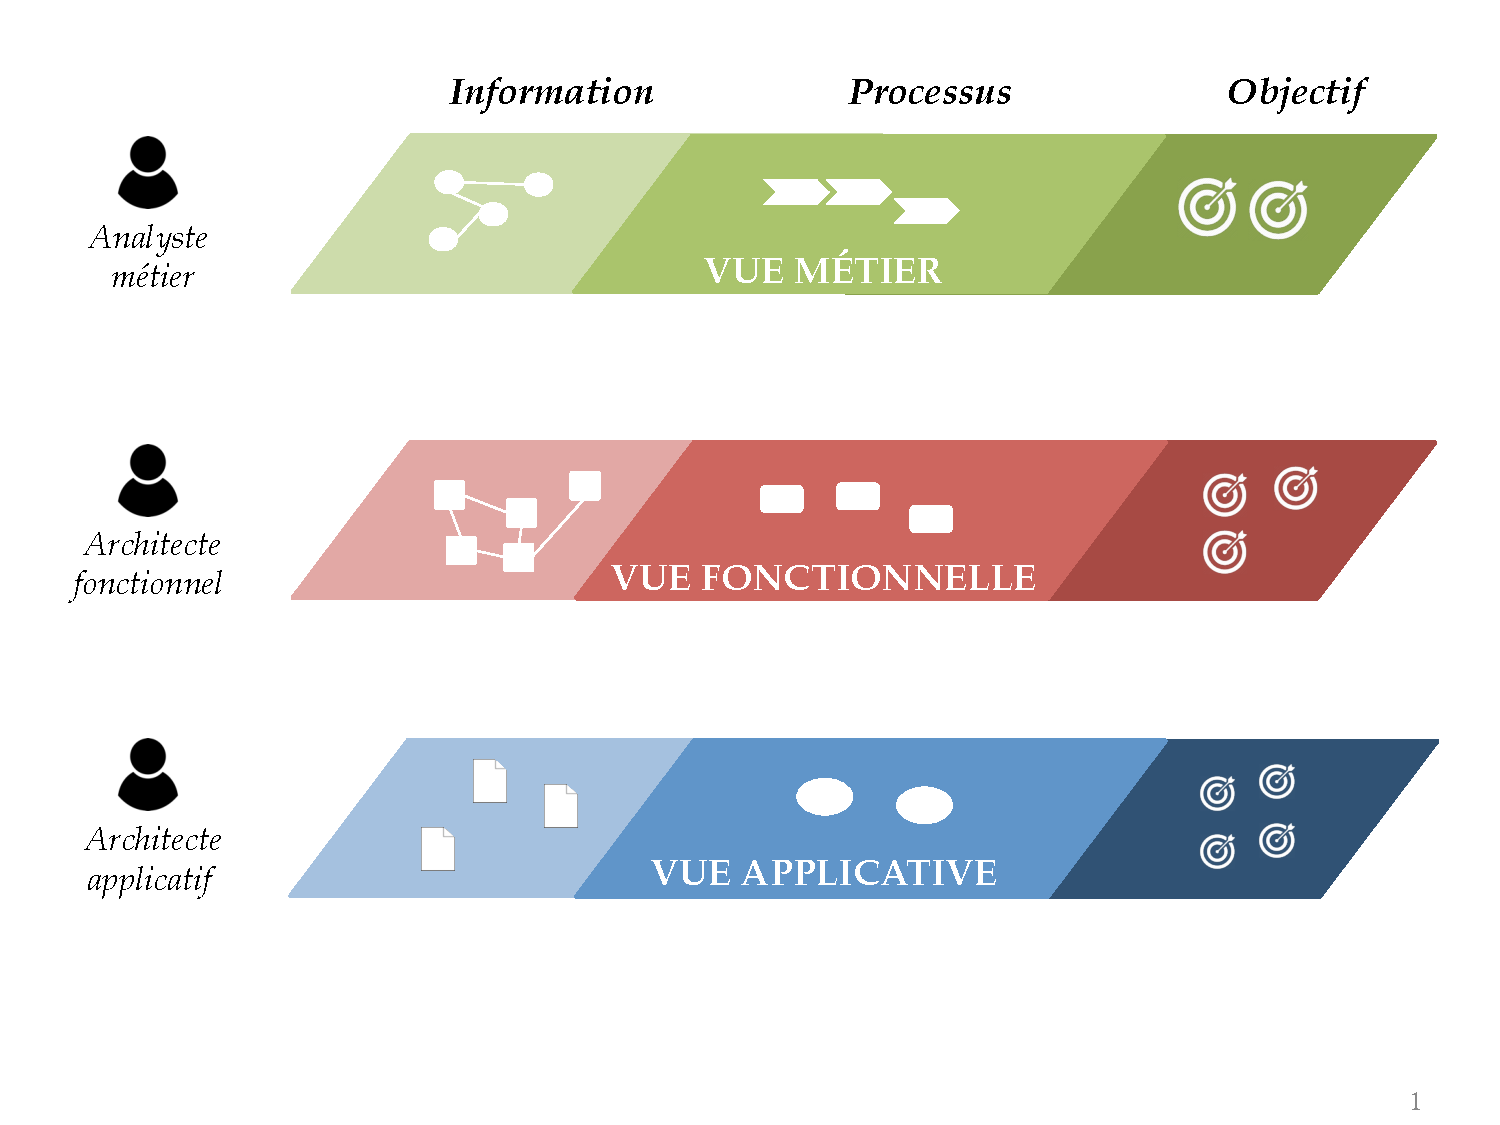
\includegraphics[trim= 0cm 3cm 0cm 0cm, width=1\textwidth]{figures/4_demarche/vue_aspect.pdf}
 \end{center}
 \caption{Points de vue et aspects utilisés}
 \label{fig:vue_aspect}
\end{figure}
	
De plus, nous modélisons le comportement de chaque vue dans l'aspect «~\textit{processus}~». Ainsi nous retrouvons~:

	\begin{itemize}
	\item \textbf{L'aspect processus du point de vue métier} 
	
	Cet aspect correspond aux processus métier de l'entreprise, décrits en utilisant les concepts métier, sans référence aux détails d'implémentation. Nous préconisons l'utilisation de formalismes standard pour la modélisation de processus métier qui soient exécutables, tels que les diagrammes d'activité fUML ou les diagrammes BPMN dans une perspective de simulation. Des langages spécifiques à un domaine (DSML) peuvent également être utilisés~;
	\item \textbf{L'aspect processus d'un point de vue fonctionnel} 
	
	Cet aspect décrit les fonctions qui réalisent les processus métier ainsi que leur orchestration en tant que processus fonctionnels. Ces fonctions sont regroupées en blocs. Chaque objet métier identifié dans l'aspect Information de la vue métier correspond à un unique bloc fonctionnel. Ceci garantit la construction de blocs fonctionnels fortement décorrélés, avec une forte cohésion interne. Dans chaque bloc fonctionnel, on retrouve les opérations correspondant à une tâche donnée du processus qui impacte l'objet métier impliqué~;
	\item \textbf{L'aspect processus du point de vue applicatif}
	
	Cet aspect décrit les modules logiciels qui implantent les blocs fonctionnels ainsi que leur orchestration en processus applicatifs. Dans un premier temps, il est conseillé de dresser un inventaire de l'existant applicatif et d'en extraire les modules capables de réaliser les opérations des blocs fonctionnels. Ensuite, si aucune application ou module existant ne peut répondre au besoin des nouveaux processus métier, l'architecte technique fait le choix des nouveaux composants applicatifs à mettre en place. En plus d'identifier les composants applicatifs existants ou à développer, l'architecte applicatif spécifie leurs interconnexions tels que échange de messages, synchronisation de données, transfert de fichiers périodique.
	\end{itemize}
	
Nous étendons chacune des vues par l'aspect «~\textit{objectif}~». Cet aspect correspond au «~\textit{pourqoi}~» du cadre Zachman qui spécifie les motivations de l'architecture. D'une part, modéliser cet aspect permet de garder une traçabilité d'une entre les processus modélisés et les objectifs qu'ils sont censés remplir. D'autre part, il permet de décliner les objectifs métier en objectifs applicatifs, et les objectifs applicatifs en objectifs fonctionnels. Comme nos travaux adoptent l'école de pensée «~Architecture du Système Entreprise~», nous souhaitons évaluer non seulement la composante SI mais l'ensemble de l'entreprise dont la stratégie. L'aspect objectif est un moyen de modéliser explicitement la stratégie de l'entreprise, traduite en un ensemble cohérent d'objectifs métier et ce pour évaluer la capacité des processus mis en place à y répondre et pour évaluer la stratégie elle-même par rapport à la réalité de l'entreprise. 

\subsection{Intégration d'une architecture d'entreprise} 

L'alignement et la cohérence sont des problématiques centrales en EA \cite{kaisler_enterprise_2005}. Notre contribution essentielle est de dédier un point de vue spécifique pour adresser ce type de problématique~:~le \textbf{point de vue intégration} illustré par la figure \ref{fig:vue_integration}. Ce point de vue définit un \textit{mapping} d'alignement en spécifiant (1)~les entités à aligner, (2)~les liens de cohérence entre ces éléments et (3) les transformations de modèles nécessaires au raffinement des ces entités. Les transformations de modèles facilitent et automatisent les passages d'une vue à l'autre. Ce point de vue permet une intégration «~IntraVue~» et «~InterVues~» (entres les aspects d'une seule vue). La figure \ref{fig:metamodele_framework} donne un métamodèle de notre framework en explicitant les concepts abordés et leurs relations.

\begin{figure}[!ht]
 \begin{center}
  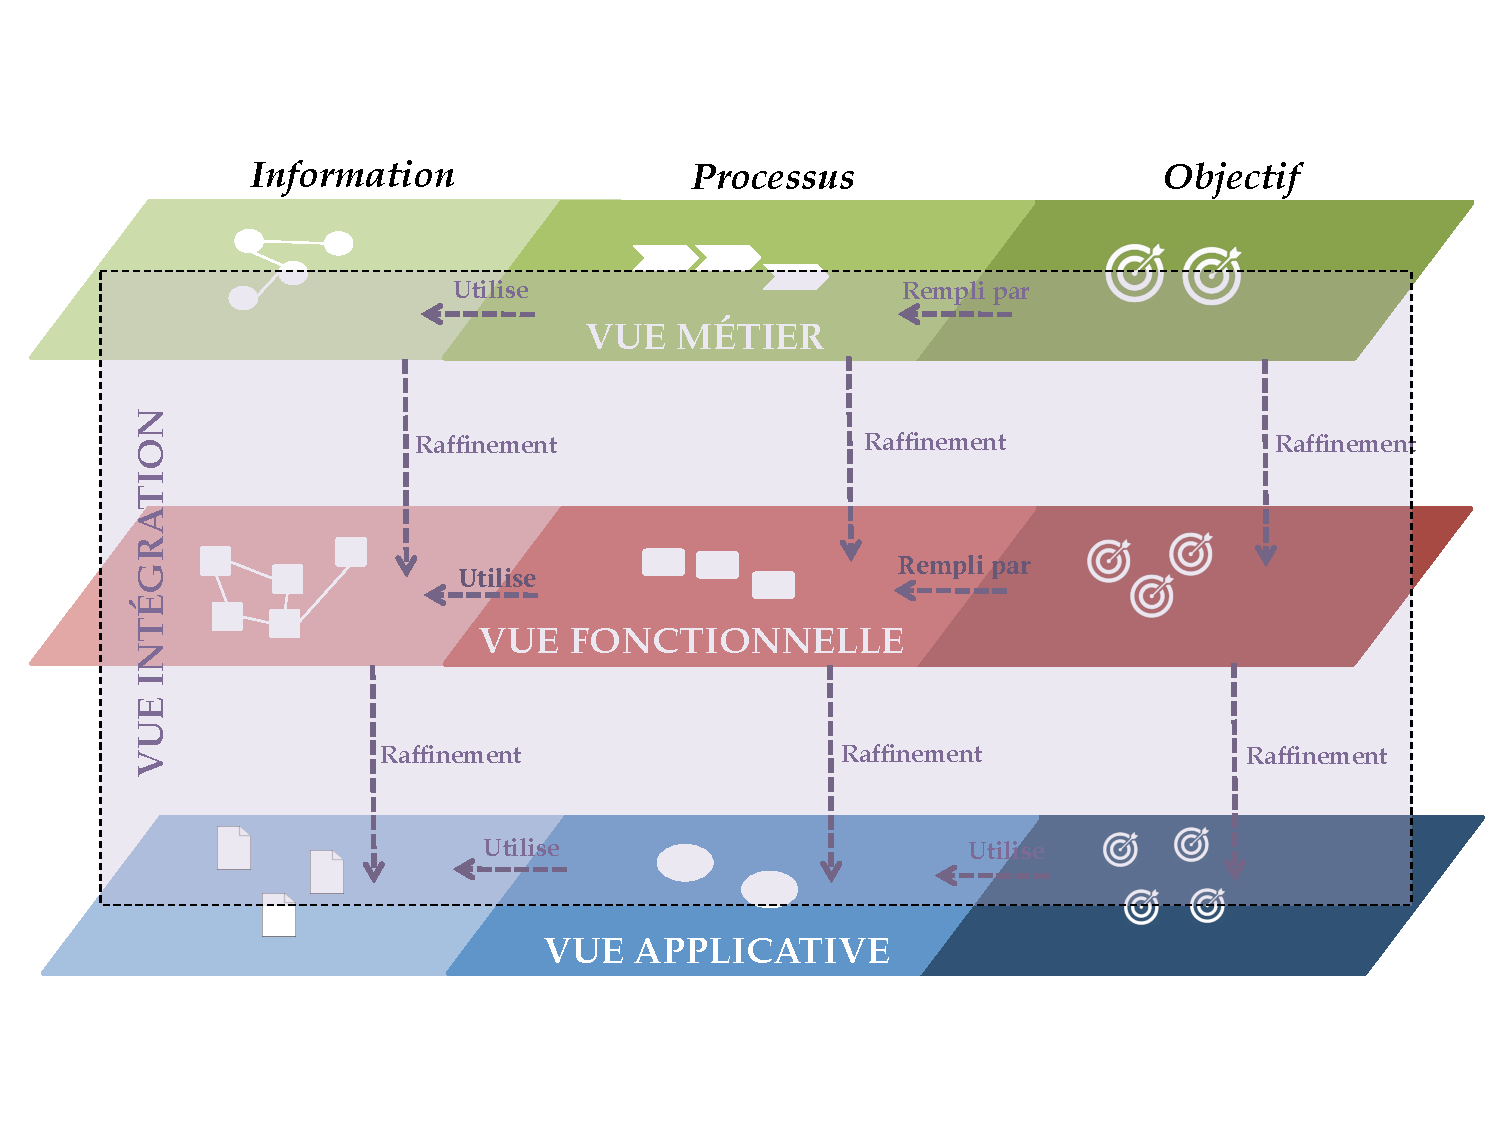
\includegraphics[trim= 3cm 3cm 0cm 0cm, width=1\textwidth]{figures/4_demarche/vue_integration.pdf}
 \end{center}
 \caption{Framework proposé avec la vue Intégration}
 \label{fig:vue_integration}
\end{figure}

L'intégration inter-vues décrit les relations entre les vues (sauf la vue intégration). La vue intégration est donc transverse à toutes les autres vues et permet de modéliser explicitement les notions de raffinement à travers la classe «~InterVues~» (voir figure \ref{fig:metamodele_framework}), tant pour  les aspects \emph{processus} et \textit{information} que sur les aspects \emph{objectif}.

\begin{figure}[!ht]
 \begin{center}
  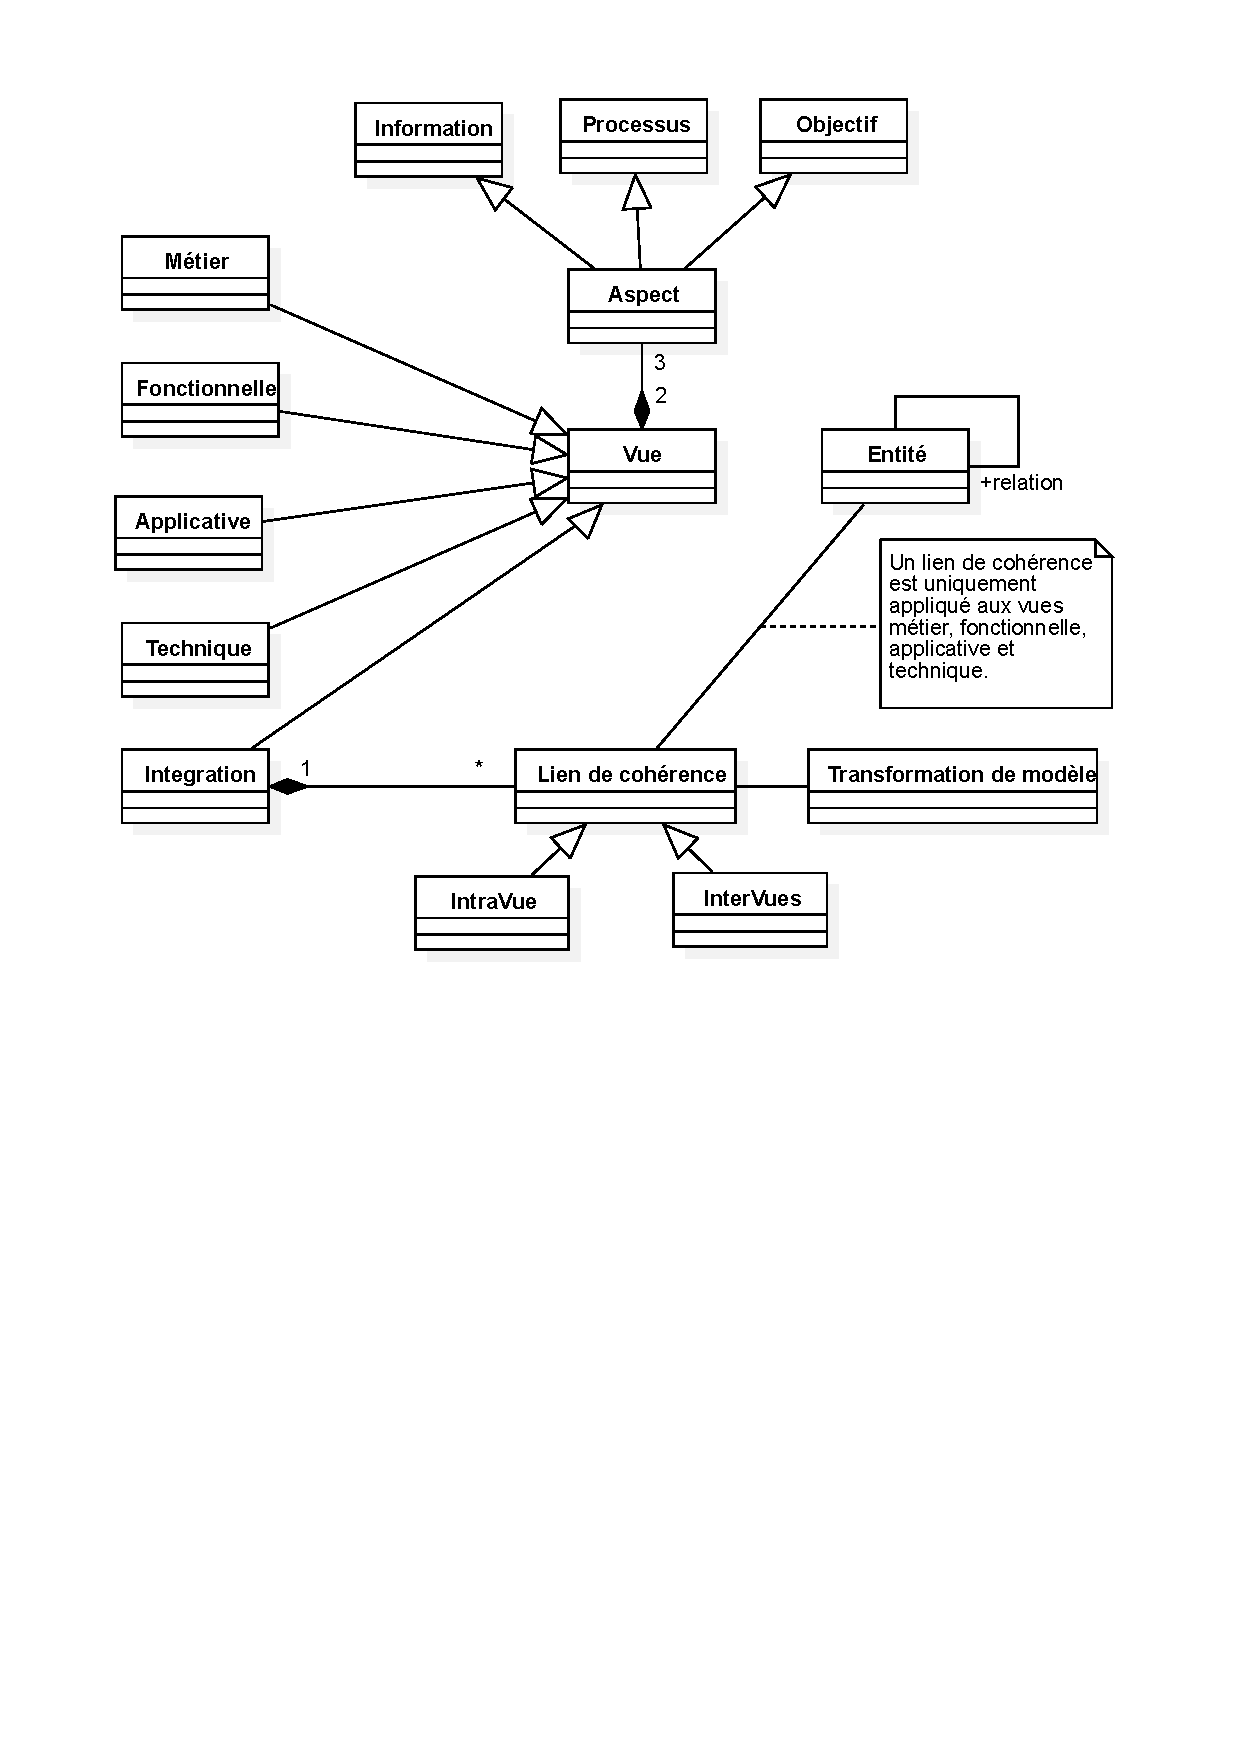
\includegraphics[trim= 0cm 13cm 0cm 2cm, width=1\textwidth]{figures/4_demarche/metamodele_framework.pdf}
 \end{center}
 \caption{Métamodèle du framework proposé}
 \label{fig:metamodele_framework}
\end{figure}

Nous donnons le métamodèle de la vue intégration dans la figure \ref{fig:metamodele_vue_integration}. Cette vue permet des vérifications horizontales à l'intérieur de chacune des vues. En effet, l'association «~utilise~» assure donc la compatibilité des données échangées entre les tâches d'un processus métier, les fonctions d'un bloc fonctionnel ou entre les modules d'une application (voir figure \ref{fig:metamodele_vue_integration}). L'association «~rempli par~» hérite aussi de la classe «~IntraVue~» et associe explicitement une entité à l'objectif qui lui est assigné. De cette manière, il est possible de tracer l'implémentation effective d'une stratégie métier à travers l'ensemble de l'entreprise, des entités métier à l'IT.

La définition d'un métamodèle précis pour le framework permet de plus de contrôler la conformité des modèles d'architecture. Ainsi, une entité du modèle (telle qu'une fonction, une tâche du processus métier, un objectif, etc.) appartient toujours à deux vues~:~une vue intégration en plus d'une autre vue parmi les vues métier, fonctionnelle, applicative et technique. Autre exemple, tous les objectifs de la vue métier doivent avoir des liens de cohérence inter-vues avec les objectifs de la vue fonctionnelle et de même pour ces dernier avec les objectif de la vue applicative et ainsi de suite. De même pour les autres entités des aspects information et processus. Une fois le modèle d'architecture créé, il est possible de vérifier sa conformité au métamodèle et de s'assurer que la cohérence entre les différentes entités de modèles est bien maintenue. 

La vue intégration permet en outre de vérifier qu'une application implémente bien tous les blocs fonctionnels nécessaires au déroulement d'un processus métier. Cette vue donne ainsi accès aux informations de traçabilité qui permettent de déterminer l'impact d'une modification ou d'une défaillance d'un module applicatif sur les processus métier. Elle permet aussi de vérifier que les formats applicatifs permettent d'encoder les types de données fonctionnelles requis, qui eux-même raffinent les concepts métiers. Cette vue détermine les éventuelles transformations de modèle nécessaires au déploiement en spécialisant l'association «~raffine~». Le choix des modèles à transformer dépend fortement de leur nature (modèles graphiques, textuels, etc.) et mais aussi de leur niveau d'abstraction. Par exemple, la génération de code demande un modèle en entrée suffisamment détaillé pour exécuter une transformation pertinente. L'état de l'art actuel des langages de transformation de modèle privilégie l'usage des transformations de modèle entre la vue fonctionnelle et et la vue applicative. 


\begin{figure}[!ht]
 \begin{center}
  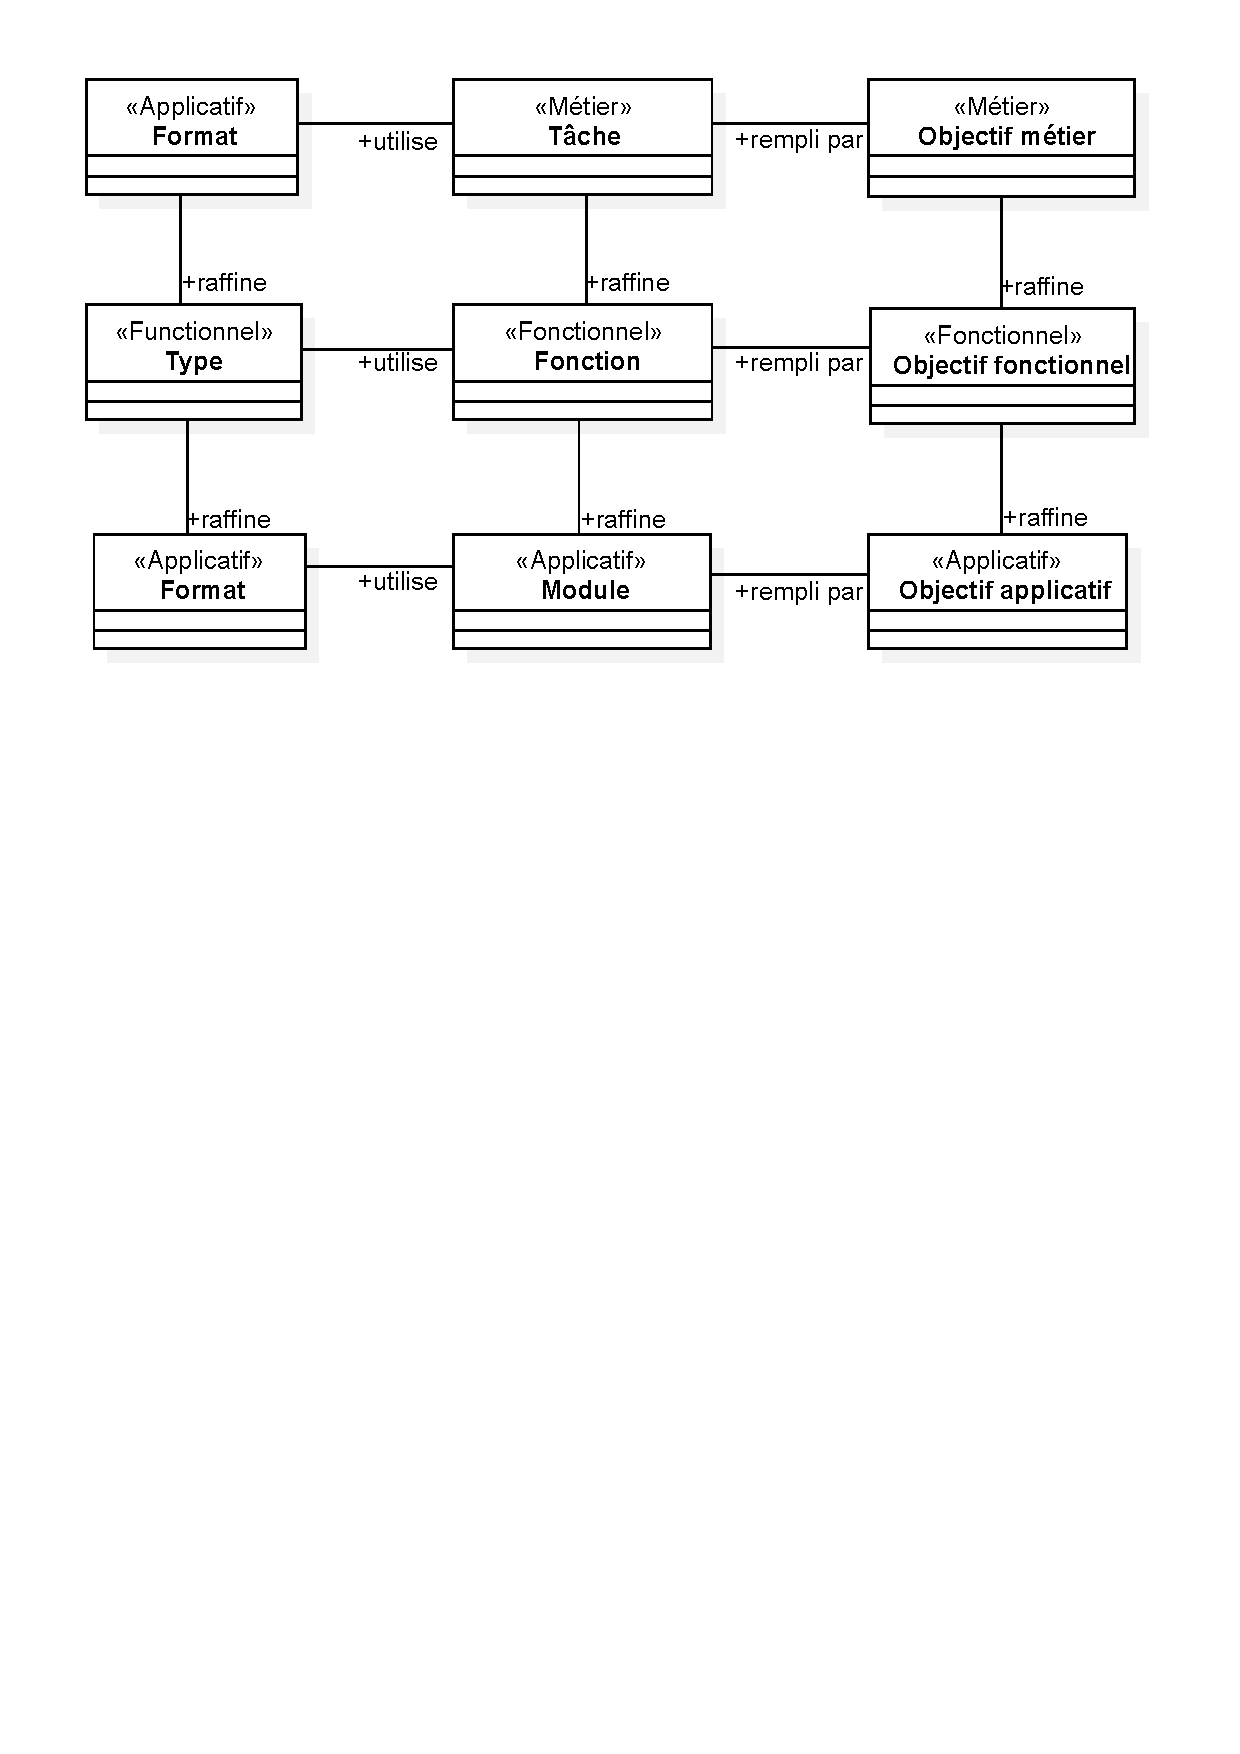
\includegraphics[trim= 0cm 18cm 0cm 0cm, width=1\textwidth]{figures/4_demarche/metamodele_vue_integration.pdf}
 \end{center}
 \caption{Métamodèle de la vue intégration}
 \label{fig:metamodele_vue_integration}
\end{figure}


\subsection{Analyse de l'architecture d'entreprise}

\subsubsection{Analyse du comportement : simulation dirigée par les processus métier}

Pour simuler le comportement d'une entreprise nous nous appuyant sur les modèles d'architecture d'entreprise préalablement définis par les différentes parties prenantes. L'EA permettent de capturer l'essentiel des composants d'une entreprise sous forme d'abstraction. Une approche par points de vue guide la décomposition d'une entreprise en vues pertinentes pour les différents acteurs. Ces vues apportent une aide supplémentaire à la définition du périmètre des modèles de simulation. La vue intégration permet en particulier de définir les liens entres les différentes vues, donc entre les différents modèles de simulation et de garantir la cohérence et donc la pertinence de la simulation. Comme les modèles de simulation sont directement dérivés de l'architecture d'entreprise telle qu'elle est définie par les parties prenantes, elle est d'autant plus facile à appréhender à comprendre. Ces derniers peuvent aussi aisément communiquer et échanger autour des résultats de la simulation. 

Les modèles d'entreprise doivent offrir un niveau d'abstraction suffisant à la compréhension, l'analyse et la communication. Les modèles doivent donc permettre d'abstraire les détails techniques et les nombreuses interconnexions tout en garantissant la traçabilité et la cohérence de l'ensemble de l'architecture. Notre approche consiste donc de mettre en lumière les composants et les relations qui sont critiques pour le comportement de l'ensemble de l'architecture. En effet, modéliser l'architecture d'une entreprise revient à la modélisation de systèmes complexes. Herbet Simon \cite{simon1990prediction} dans ses travaux de modélisation de systèmes complexes affirme que «~l'approximation judicieuse et non la puissance de calcul d'une machine~» reste la manière la plus effective d'adresser des systèmes complexes.

La simulation des processus métier est souvent réduite à de la simple animation visuelle de diagrammes pour vérifier l'orchestration des taches métier. Nous proposons de piloter la simulation du comportement de l'architecture par le processus métier. Dans ce cas, le calcul d'une valeur ne se fait pas au niveau de la tache métier mais du module applicatif qui l'implémente. Le processus métier est modélisé sous forme de diagrammes d'activité fUML. Dans ce cas les simulations du comportement de l'architecture d'entreprise est pilotée par les processus métier qui sont alors responsable d'orchestrer l'ensemble des modèles comme l'illustre la figure \ref{fig:Simulation_Approche}. La simulation est lancée après l'intégration de l'architecture à travers la création de lien de cohérences intra-vue et inter-vues. Ces liens sont par la suite utilisés pour mettre en œuvre la simulation. D'une part, la \textit{Tâche~A} de la figure \ref{fig:Simulation_Approche} appelle le \textit{Module~A} car le \textit{Module~A} raffine la \textit{Fonction~A} qui elle-même raffine la \textit{Tâche~A}. D'autre part, les liens de cohérences intravue garantisse une compatibilité entre les informations envoyés par la \textit{Tâche~A} et celles attendues par la \textit{Tâche~B}, de même entre la \textit{Fonction~A} et la \textit{Fonction~B} et entre le \textit{Module~A} et le \textit{Module~B}.

\begin{figure}[!ht]
 \begin{center}
  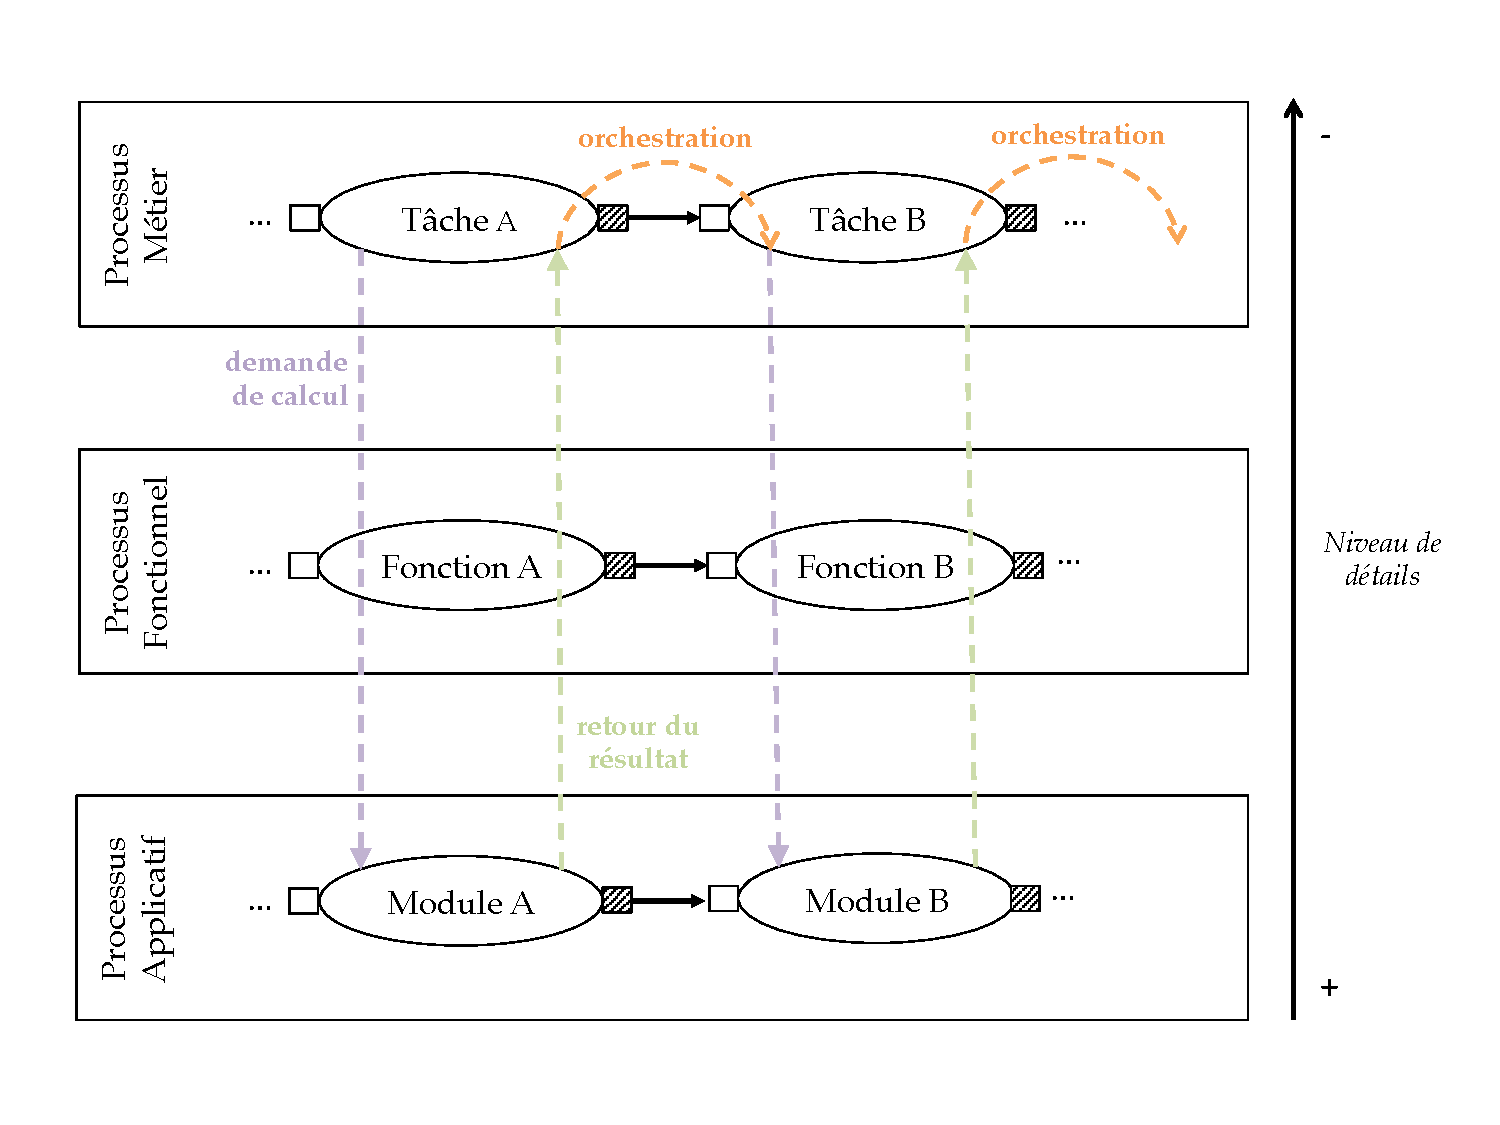
\includegraphics[trim= 0cm 2cm 0cm 0cm, width=1\textwidth]{figures/4_demarche/approche_simulation.pdf}
 \end{center}
 \caption{Simulation dirigée par les processus métier}
 \label{fig:Simulation_Approche}
\end{figure}

En plus de s'appuyer sur les processus métier pour piloter la simulation de l'ensemble du comportement de l'architecture d'entreprise, notre approche consiste à mettre à profit les techniques et les langages de l'IDM pour faciliter l'automatisation de l'activité d'analyse du comportement. Nous nous appuyant sur le manifesto de IBM \cite{chesbrough2006research} concernat l'IDM dans la sélection de techniques et langages qui soient pertinents pour notre approche. Le mnifesto de IBM recommande l'utilisation de langages (1)~exécutables, (2)~standardisés et (3) compréhensibles par les experts du domaine. C'est le cas de fUML, BPMN et OCL. La figure \ref{fig:IDM_EA} fait la correspondance entre les langages et la possibilité de les utiliser selon les vues. 


Ces langages permettent une exécution directe des modèles créés. Contrairement à d'autres méthodes de simulation de processus métier qui utilisent l'IDM pour isoler la définition du processus de son exécution. Ces méthodes font ensuite appel aux transformations de modèle pour automatiser la conversion entre les modèles de représentation et leur exécution. 

\begin{table}[!ht]
    \begin{center}
        \setlength{\mytablewidth}{0.8\textwidth}
\setlength{\mycolwidth}{\dimexpr0.25\mytablewidth-2\tabcolsep\relax}

\begin{tabulary}{\mytablewidth}{m{\mycolwidth}m{\mycolwidth}m{\mycolwidth}m{\mycolwidth}}
\cmidrule[\heavyrulewidth]{2-4}

                        & \centbf{Metier}       & \centbf{Fonctionnel}  & \centbf{Applicatif}   \tabularnewline\midrule
    \centbf{BPMN}       & \center{\checkmark}   &                       &                       \tabularnewline
    \centbf{fUML}       & \center{\checkmark}   & \center{\checkmark}   &                       \tabularnewline
    \centbf{OCL}        &                       & \center{\checkmark}   &                       \tabularnewline
    \centbf{MiniZinc}   &                       &                       & \center{\checkmark}   \tabularnewline

\bottomrule
\end{tabulary}

    \end{center}
    \caption{Langages de l'IDM pour l'EA}
    \label{fig:IDM_EA}
\end{table}

\subsubsection{Analyse de la structure}
Tout comme l'analyse du comportement, l'analyse de la structure de l'architecture d'entreprise est étroitement lié à l'impératif de cohérence.  Il est indispensable s'assurer de la cohérence entres les modèles des différentes vues avant d'initier une analyse structurelle qui soit pertinente pour les parties prenantes et en particulier pour l'architecte d'entreprise. 

Notre contribution consiste à définir la manière dont les langages et techniques de l'IDM peuvent être utilisés pour mener une analyse structurelle des modèles d'entreprise. Le cadre d'EA que nous proposons permet d'acquérir une vision globale et cohérente de l'ensemble des artefacts qui la composent. La taille de plus en pls importantes des entreprises actuelle fait que la complexité de l'entreprise en tant que système se retrouve dans les modèles d'architecture qui le représentent.

L'analyse automatisée de ces modèles facilite leur appréhension par l'acteur qui mène ces analyses (en l'occurrence l'architecte d'entreprise). Elle permet de révéler la structure de l'entreprise et le fonctionnement de cette structure. Un intérêt  typique de l'analyse de la structure est la mesure de l'impact du changement \cite{de2005change} sur l'architecture. L'analyse de l'impact du changement consiste à dévoiler les effets de bord d'un changement apporté à un élément de l'architecture.  

Les langages de modélisation doivent donc permettre de représenter convenablement les différents composants de l'entreprise en plus d'offrir la possibilité d'analyser la structure des modèles créés dans l'objectif de mieux comprendre le système réel, qui est dans ce cas l'entreprise. Nous proposons donc de tirer profit des méthodes IDM telle la métamodélisation et de les associer à des langages capables d'exprimer et d'exécuter des contraintes et des requêtes sur les modèles tels que OCLinEcore ou QVT. Grâce à ce type de langage il est possible de~:
\begin{enumerate}
\item modéliser des règles de structure supplémentaires qui précisent d'avantage méta-modèle d'architecture. Une fois que le modèle d'architecture est conforme à ce métamodèle, il est possible de vérifier qu'il respecte bien toutes les contraintes exprimées au niveau du métamodèle~;
\item analyser l'impact du changement pour évaluer par exemple l'impact de l'indisponibilité d'un module applicatif sur l'architecture globale. En mettant à profit les liens de cohérence de la vue intégration, il est alors possible de déterminer quels sont les processus métier ou fonctionnels touchés par cette défaillance applicative. De même, il est possible d'identifier les modules applicatifs existants pouvant participer à la réalisation d'un nouveau métier si ces processus fait intervenir des taches métier déjà implémentées dans le SI.
\end{enumerate}




 

%(Describes the system’s functional elements, their responsibilities, interfaces, and primary interactions. A Functional view is the cornerstone of most ADs and is often the first part of the description that stakeholders try to read. It drives the shape of other system structures such as the information structure, concurrency structure, deployment structure, and so on. It also has a significant impact on the system’s quality properties such as its ability to change, its ability to be secured, and its runtime performance.)

%\subsubsection{Le Model Typing pour la cohérence inter- et intra-vue}
%Le \textit{Model Typing} est une technique de l'IDM appliqué au développement logiciel permettant de contrôler les types de modèles d'entrée des transformations de modèle à leur exécution. Nous proposons d'appliquer les principes du \textit{Model Typing} aux modèles d'EA et aux transformations de modèle qui leurs sont associées. Par exemple, un processus métier utilise en entrée et en sortie des modèles représentant des concepts métier. Un processus peut donc être considéré comme une transformation de modèle. 
%Ainsi, le \textit{Model Typing} peut être utilisé pour l'intégration horizontale (i.e. cohérence et orchestration des processus d'une même vue). 





